\section{Introduction}
\label{sec:intro}
%Charmed baryons provide an unique laboratory to study the strong and weak interactions. Its hadronic decays happen only through the weak interaction. Many theoretical efforts, including the covariant confined quark model~\cite{Korner:1992wi,Ivanov:1997ra}, the pole model~\cite{Cheng:1991sn,Xu:1992vc,Cheng:1993gf,Xu:1992sw,Zenczykowski:1993jm,Sharma:1998rd}, current algebra~\cite{Korner:1978ec,Uppal:1994pt}, and the SU(3) flavor asymmetry approached, have been put to describe properties of charmed baryons. However, the predictions are very difficult due to the contributions of the non-factorizable processes arising from the W-exchange and inner W-emission diagrams. The experimental studies of charmed baryons are crucial to give constraints on the theoretical models.
Study of charmed baryons provides is an important tool to understand the fundamental theory of the strong and weak interactions of particle physics. Comparing to the charmed mesons,The progresses from both theoretical and experimental side are slow until 2014, when the BESIII started the data-taking around the $\lcp\lcm$ energy threshold. Although the theoretical interest lasts a long time, there is still no good and reliable phenomenological models to describe the properties and decay dynamic mechanisms of charmed baryons. The experimental studies of charmed baryons are crucial to give constraints and provide inputs for the the proposed theoretical models. 

One of the unique advantages of the $\ee$ experiments of modern facilities is to produce baryon and antibaryons with unprecedented intensity and clean backgrounds. The baryon-antibaryons pair are produced through a single photon annihilation or other resonances, such as charmoninum states. The Born cross section for the process $e^+e^- \to B\bar{B}$, where $B$ represents a spin-$1/2$ baryon, can be parametrized as functions of electromagnetic form factors (EMFFs), i.e. $G_E$ and $G_M$, as follows:
\begin{equation}
\sigma_{B\bar{B}}(s) = \frac{4\pi\alpha^2C\beta}{3s}|G_M(s)|^2\left( 1 + \frac{2m_B^2c^4}{s}|\frac{G_E(s)}{G_M(s)}|^2\right),
\end{equation}
where $\alpha$ is the fine-structure constant, $\beta$ is the velocity of the baryon, $s$ is the square of center-of-mass (c.m.) energy and $m_B$ stands for the mass of the baryon~\cite{Cabibbo:1961sz}. The electromagnetic structure of baryons can be probed by the EMFFs, which provide a key to understanding the Quantum chromodynamics effects. As the electromagnetic process obeys parity conservation, the longitudinal polarization of the baryon is absent. Nevertheless, transverse polarization emerges spontaneously due to the non-vanishing phase angle difference between $G_E$ and $G_M$, which can be derived from the independent helicity amplitudes in the $e^+e^- \to B\bar{B}$ reaction.  

BESIII has observed the polarization effects of baryons in the processes of  $J/\psi \to \Lambda\bar{\Lambda}$~\cite{BESIII:2018cnd,BESIII:2022qax}, $e^+e^-\to\Lambda\bar{\Lambda}(\sqrt{s}=2.396\gev)$~\cite{BESIII:2019nep}, $J/\psi$ and $\psi(3686) \to \Sigma^+\Sigma^-$~\cite{BESIII:2020fqg}, $\psi(3686) \to \Xi^-\bar{\Xi}^+$~\cite{BESIII:2022lsz} and $J/\psi \to \Xi^0\bar{\Xi}^0$~\cite{BESIII:2023drj}. Additionally, BESIII has conducted measurements of the polarization and decay asymmetry parameters of baryons in processes such as $\psi(3686) \to \Xi^0\bar{\Xi}^0$~\cite{BESIII:2023lkg} and $J/\psi \to \Xi^-\bar{\Xi}^+$~\cite{BESIII:2021ypr}. The baryon's polarization is expected to be along the normal of production plane, and can be accessible through the angular distributions of decay products of the baryons. The polarization is characterized by the relative phase between transition amplitudes of the baryon-antibaryon pair. Similarly, in the process of $e^+e^- \to \Lambda_c^+\Lambda_c^-$, the $\Lambda_c^+\Lambda_c^-$ pair are expected to have a non-zero transverse polarization  perpendicular to the production plane. Its nominal value is characterized by:
\begin{equation}
    P_T = \frac{3}{2(3+\alpha_0)}\sqrt{1-\alpha_0^2}\sin\Delta_0\cos\theta_{\lcp}\sin\theta_{\lcp},
    \label{eq:eq_polar}
\end{equation}
where $\alpha_0$ and $\Delta_0$ represent the ratio and phase angle difference between $G_E$ and $G_M$, respectively~\cite{Chen:2019hqi}. The helicity angle $\theta_{\Lambda_c^+}$ is defined as illustrated in Figure~\ref{fig:helicity_ee_lclp}. In the language of helicity formalism, the baryon-antibaryons have only two independent helicity states, $H_{\frac{1}{2},-\frac{1}{2}}$ and $H_{\frac{1}{2},\frac{1}{2}}$. The EMFFs are related to the helicity as
\begin{equation}
    \begin{split}
        G_E(s) &= \frac{1}{2m_{\lcp}}H_{\frac{1}{2},\frac{1}{2}}, \\
        G_M(s) &= -\frac{1}{\sqrt{2}s}H_{\frac{1}{2},-\frac{1}{2}},
    \end{split}
\end{equation}
The helicity amplitudes $H_{\frac{1}{2},-\frac{1}{2}}$ and $H_{\frac{1}{2},\frac{1}{2}}$ in $e^+e^- \to \Lambda_c^+\Lambda_c^-$ are used to express $\alpha_0$ and $\Delta_0$:
\begin{equation}
    \begin{split}
    \alpha_0 &= \frac{|H_{\frac{1}{2},-\frac{1}{2}}|^2 - 2|H_{\frac{1}{2},\frac{1}{2}}|^2}{|H_{\frac{1}{2},-\frac{1}{2}}|^2 + 2|H_{\frac{1}{2},\frac{1}{2}}|^2}, \\
    \Delta_0 &= \mathrm{arg}(H_{\frac{1}{2},-\frac{1}{2}}) - \mathrm{arg}(H_{\frac{1}{2},\frac{1}{2}}),
    \end{split}
    \label{eq:eq_alpha_delta0}
\end{equation}
where subscripts ($\frac{1}{2}$, -$\frac{1}{2}$) and ($\frac{1}{2}$, $\frac{1}{2}$) denote the same or opposite helicity of $\lcp\lcm$ pair.
In the amplitude analysis, the helicity amplitude can be further expanded using LS coupling to
\begin{equation}
    \begin{split}
        H_{\frac{1}{2},\frac{1}{2}} = \frac{g_{0,1}}{\sqrt{6}} - \frac{g_{2,1}}{\sqrt{3}}, \\
        H_{\frac{1}{2},-\frac{1}{2}} = \frac{g_{0,1}}{\sqrt{3}} + \frac{g_{2,1}}{\sqrt{6}},
    \end{split}
    \label{eq:eq_helicity}
\end{equation}
where $g_{0,1}$ and $g_{2,1}$ are the complex amplitudes and subscripts denote $ls$ combination of $\lcp\lcm$ pair.

\begin{figure}[htbp]
    \centering
    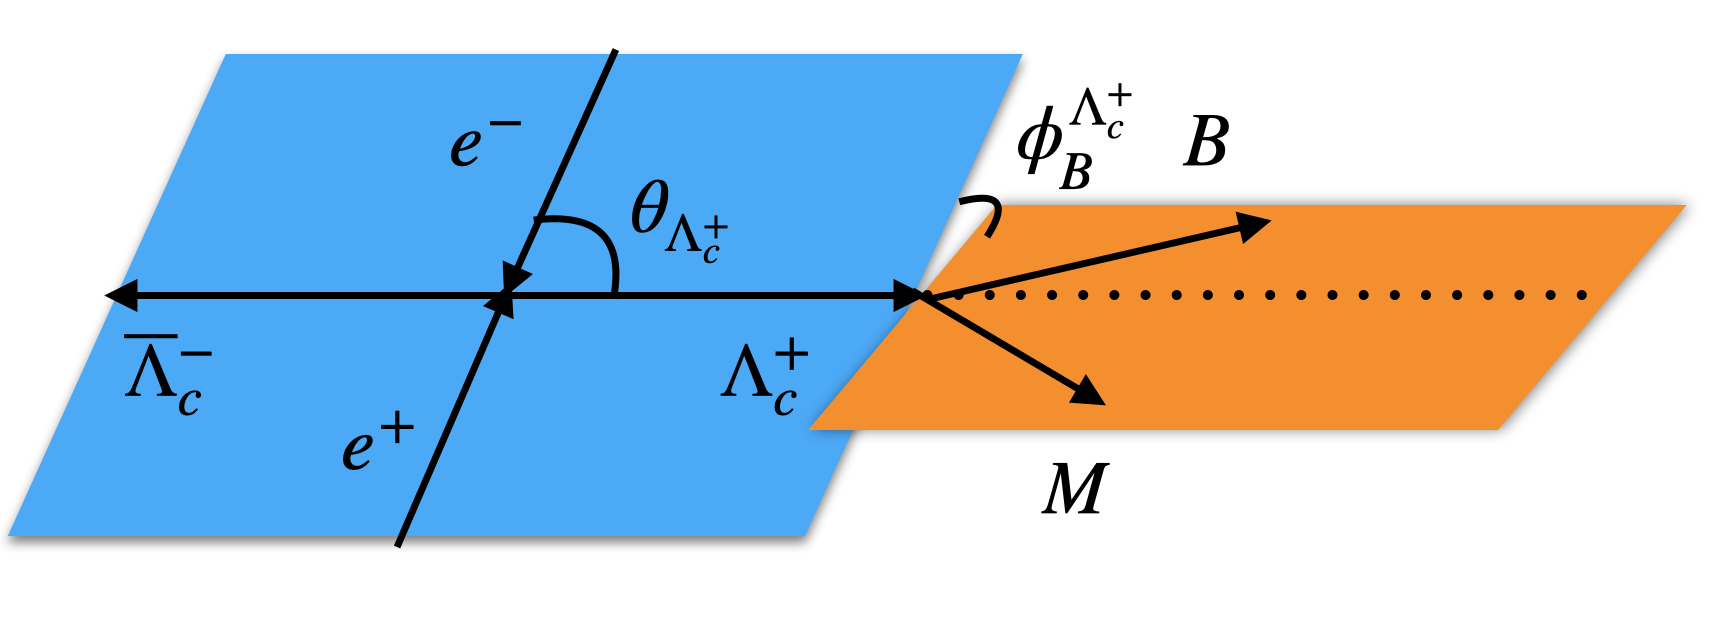
\includegraphics[width=0.50\textwidth]{figure/helicity.png}
    \caption{Definition of helicity angle in the process of $e^+e^- \to \lcp\lcm$ and $\lcp \to BM$. $B$ and $M$ denotes baryon and meson in the decay of $\lcp$. $\theta_{\lcp}$ is the angle between the $\lcp$ and $e^+e^-$ in the rest frame of $e^+e^-$. $\phi_{B}^{\lcp}$ is the angle between the production plane of $\lcp$ and plane determined by the decay products of $\lcp$.} 
    \label{fig:helicity_ee_lclp}
\end{figure}

In this analysis, we perform a amplitude analysis for $e^+e^- \to \lcp\lcm$, $\lcp \to p K^- \pi^+$ and $\lcm$ decays inclusively, using data samples collected at thirteen center-of-mass energies from 4.600 to 4.951 GeV with the BESSIII detector at BEPCII. The charge conjugation is always implied. The transverse polarization parameters, $\alpha_0$ and $\sin\Delta_0$ are obtained at each energy points. Based on the amplitude analysis results of $\lcp \to pK^-\pi^+$, the composition of the resonance structures are obtained in the $pK^-\pi^+$ final state. The decay asymmetry parameters of quasi-two-body $\lcp$ decay are also provided.
